\chapter{Introduction}

\section{Background}
Looking at renting in the student accommodation industry, specifically on the ability to accurately forecast revenue using the data stored in the property management system (\cite{Jain2006IntellectualPerspective}). This will be done by using machine learning to predict under what circumstances a contract will not be fulfilled.

\vspace{5mm}

A contract made in advanced between the student (customer) and the company defines the services that will be sold (the room) as well as the start and end date of the tenancy and the fix price the service will be sold at. In the case of student accommodation this contract is usually made a few months in advanced, in some cases before the student has finalized there plan to attend a specific university. Because of this the student withholds the right to cancel the contract before it is paid. The inherit uncertainty of the contract means there is no way for the company to definitively measure what the occupancy and sales of a given property will be in advanced since they have to take on the risk. This problem is not specific to the student accommodation industry, this is a problem of revenue management first identified by the aviation industry in 1966  (\cite{Chiang2007AnResearch})


\subsection{Problem Statement}

In total for the year 2020 to 2021, 25 percent of all 14363 bookings made where cancelled, this accounts for over 20 million pounds in revenue loss from customers who completed there booking then cancelled before the contract was payed. There are a number of different reasons that account for each booking being cancelled that range from impact caused due to COVID and students not receiving there target grades. In most of these cases the student will then chose to stay at different accommodation meaning the sale has been lost. Producing a model that is able to predict which of these bookings will be cancelled in real time would then allow the business to take actions to try and prevent the student from cancelling there booking. Being able to prevent just 10 percent of users from cancelling would therefore create a potential gain of 2 million in revenue per year.  

\vspace{5mm}

On a small scale it would be relatively easy for a human to identify the attributes common with bookings that would then be canceled, for example looking at the percentage of bookings canceled in the previous year. In this case however when the company operates over 70,000 beds across the world it is clear that no amount of human analysis would be able to take into account that many variables. 

\vspace{5mm}

\textbf{this paragraph is mostly a repeat of the 2nd paragraph}The fact that when a booking is made the student maintains the ability to cancel it up until a given time period for a given penalty means that it is the providers responsibility to account for the inherit uncertainty of the agreement. There's a number of different ways this problem can be solved that should take into account all of the possible variables, usually this is done by simply taking the number of bookings canceled in the previous year then using this number as an average to calculate the number of bookings likely to be canceled in the current year. The problem with this method is that it only takes into account one of the many variables (previous year figures) when in reality the business stores hundreds of data points on each of the bookings made.

It is for this reason I am attempting to solve this problem using machine learning

Since the dataset I am using is coming directly from the company in question and contains real data about students I have taken out all personal information I will be referring to students and properties only by there ID so that the company and students remain anonymous. 
    
\section{Aims and objectives}
The aim is to predict with some degree of certainty which of the bookings currently made and any new bookings will be cancelled by inputting all data points from all of the previous years bookings that have known outcomes, I hope to produce a model that can classify a booking made into 2 distinct states, cancelled or not cancelled.

It is important to not just create a model that will predict which bookings will be cancelled but also to understand why bookings are cancelled by using the model to identify which features in the dataset have the most affect on weather or not the customer will cancel. Doing this is important in helping the company to make business decisions on the data to not only prevent the cancellation from occurring but to understand what actions can be taken that will reduce the number of cancellations made in the future.  

The first stage to any machine learning problem is obtaining accurate and clean data, in most cases (including this one), this is the hardest problem to solve as data is not usually stored in a way that makes it easy to read and analyse, most of the time data is stored  then never used. For this reason I am approaching the problem by building a data warehouse to properly store and analyse the data before building a classification model [\textbf{reference supporting why accurate data is important}]. This data warehouse will exist in the Azure cloud on top of Docker Containers with the code written in python, with the aim being to create a stream to import new booking data into the data warehouse hourly ensuring that it is stored in a way that makes it easy to use for model training

The aim is to integrate the classification model into the booking management system by creating a daily list of which customers are most likely to cancel there bookings to the managers of there respective properties along with the recommended actions to be taken to prevent the cancellation. Storing the data of the actions taken and weather or not it was successful will then be used to improve future iterations of the model

\begin{itemize}
\item maybe create an image of how this would look
\end{itemize}



\section{Solution approach}

To understand what the best way to approach the solution to the problem would be I started by working with employees in the company to gain a better understanding of what kind of results would be most effective and what are the actions that can be take to have the best chance of preventing a cancellation from being made at the level of an individual booking. It is important the results can be displayed in a way that is easy for employees to understand so that actions can be taken easily. I found that the best way to display the results of the model would be to create a table that ranked bookings by highest probability of cancellation. Another feature I found to be important is the ability to retrain the model on new data and adjust the hyper tuning parameters.
\begin{itemize}
\item explain this better
\end{itemize}
To do this I will be using the cross industry standard process for data mining (CRISP-DM)


\vspace{5mm}

begin{figure}[hbt!]
 %\centering
 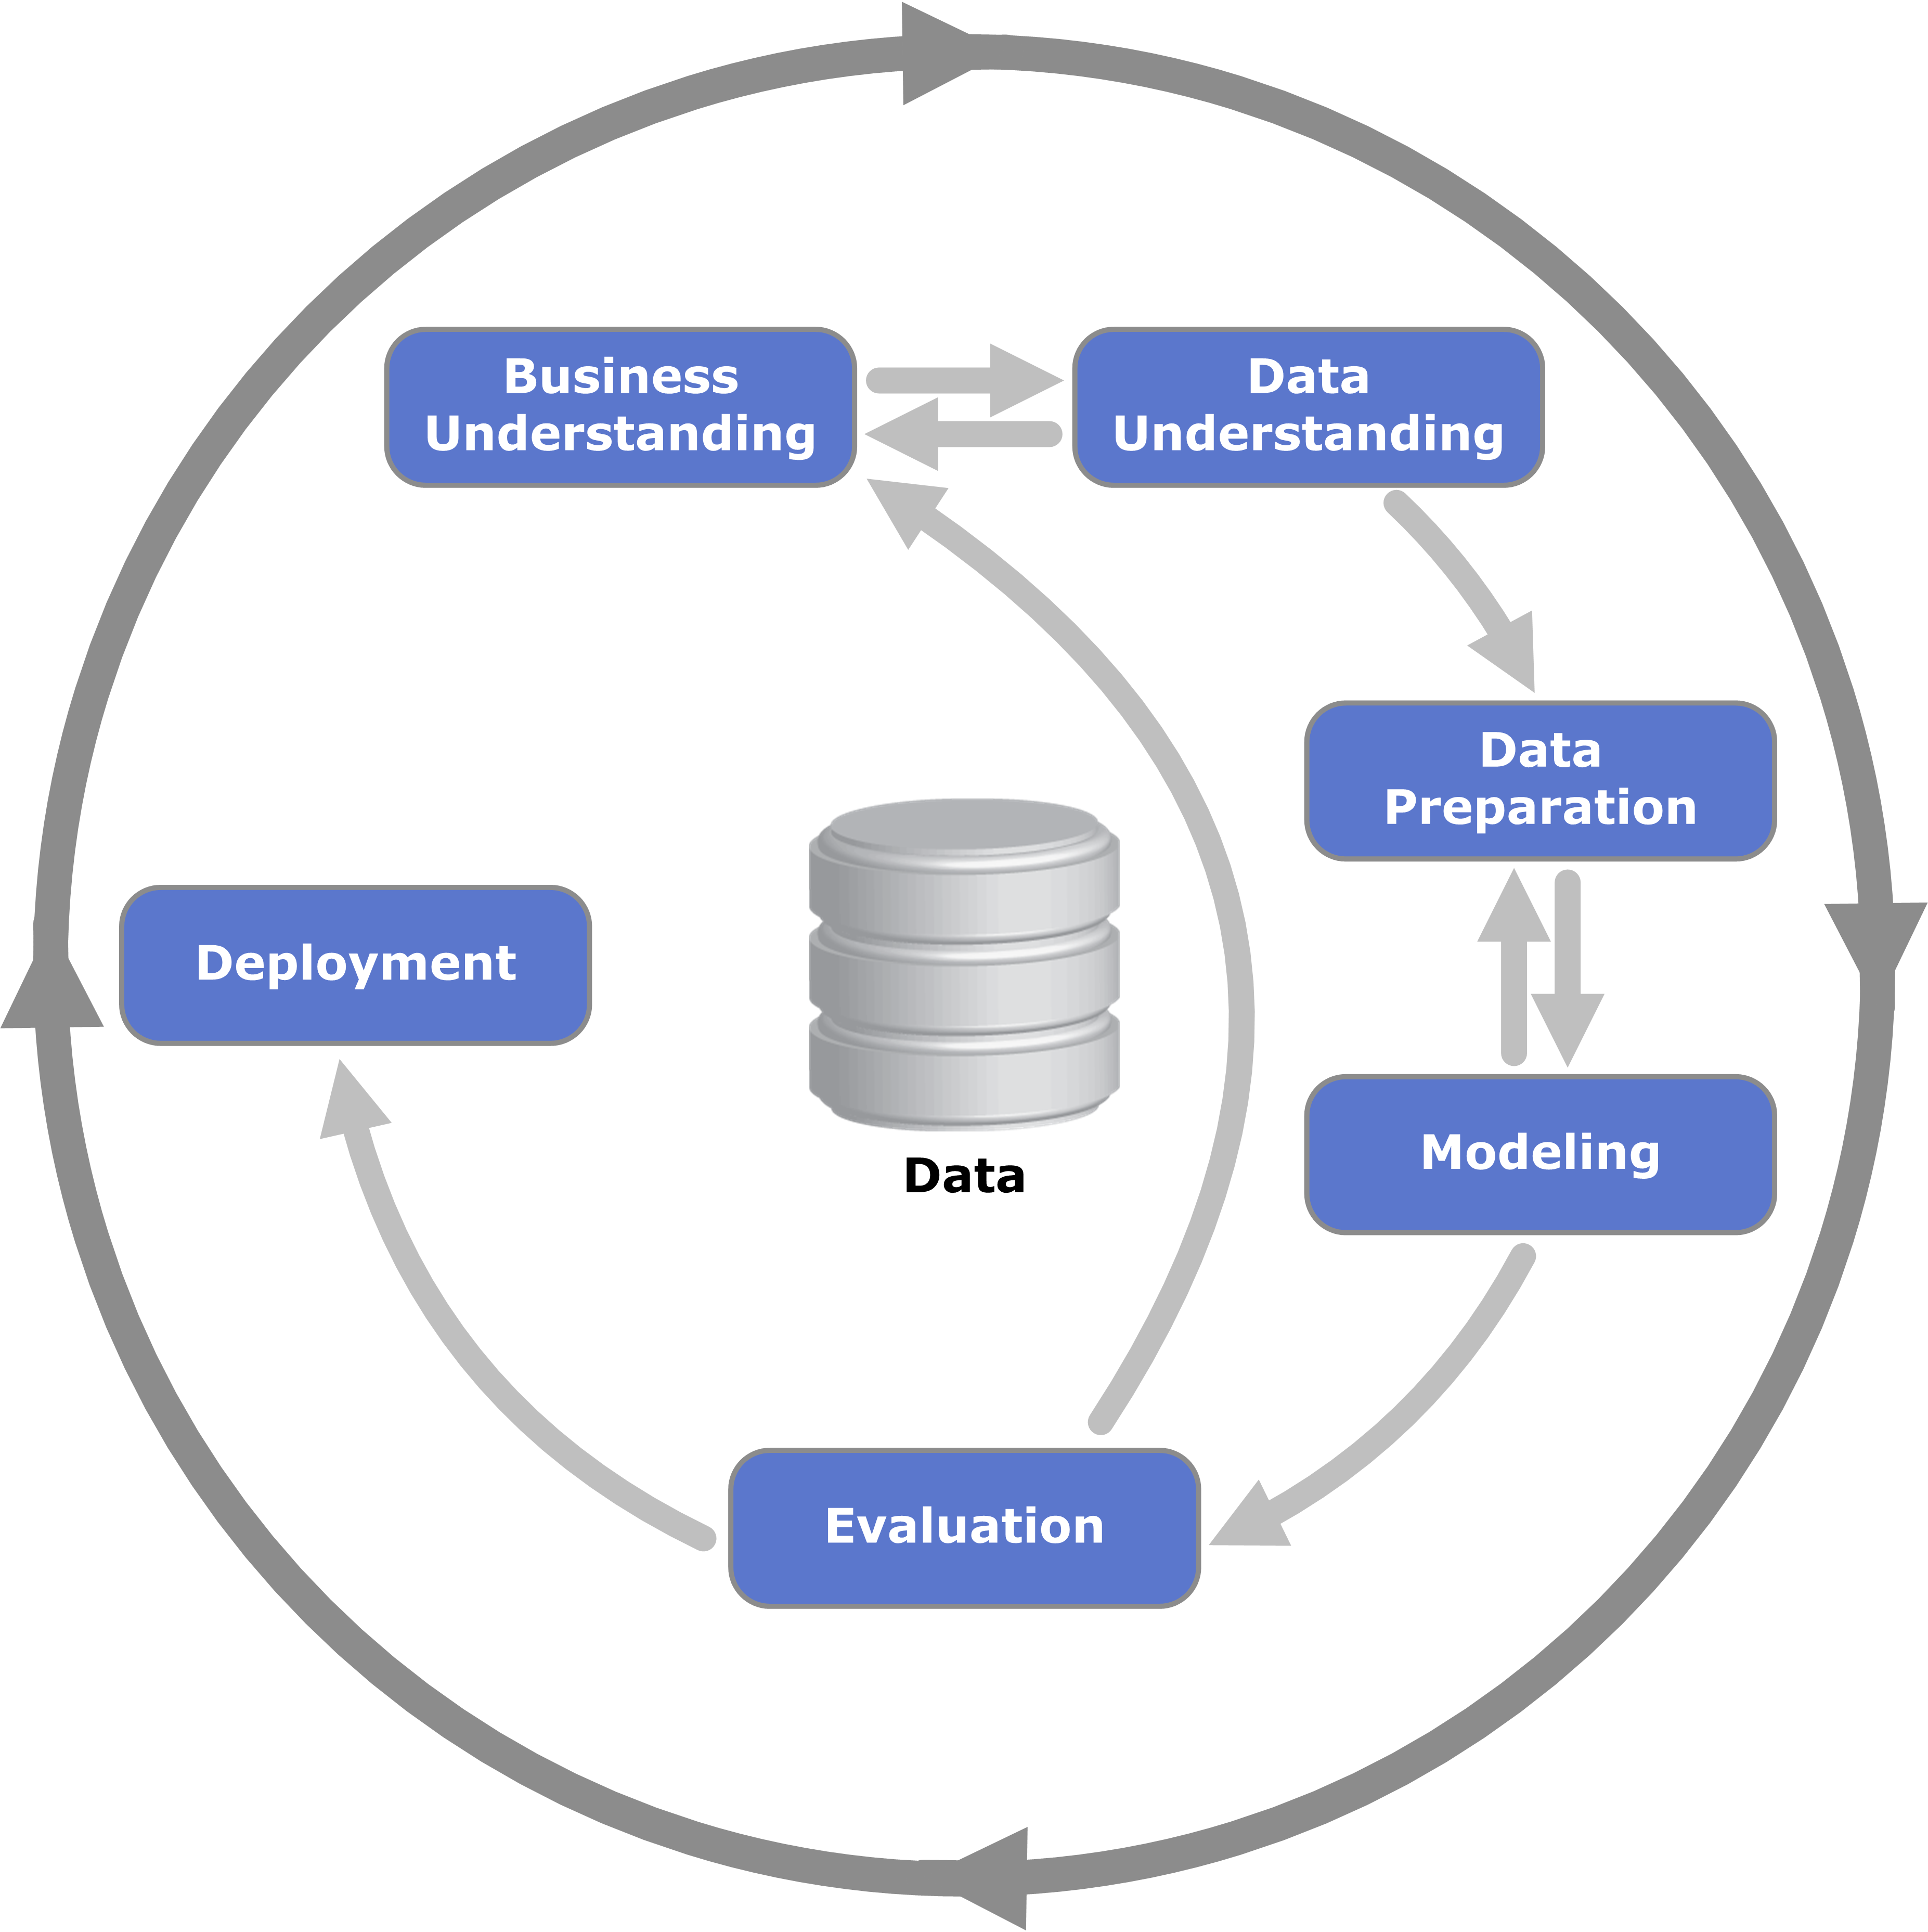
\includegraphics[width=10cm]{figures/CRISPDM_Process_Diagram.png}
 \caption{https://www.datascience-pm.com/crisp-dm-2/}
\end{figure}



For this paper I will be creating a single model using the Azure ML studio to find if it is able to make accurate predictions on the data. I am using Azure ML because it provides the functionality to deploy models onto a cloud environment that can be easily integrated into the booking management system through the provided API . It also allows for easier retraining on the model after the evaluation stage while testing a number of different regression models each time and selecting the one with the highest accuracy. For this paper I will only be testing the model first iteration of the model 

\begin{itemize}
\item working with the company to understand what the requirements are, how cancellations predictions will be used, how results will be displayed to employees
\item why modeling needs to be fast and dynamic 
\item why building a data warehouse was important to solving the problem, since having the ability to retrain the new model is essential 
\item CRISP-DM, this is an iterating process of modeling an evaluation of the model
\item this entire process will be done in the azure cloud using technologies such a Python, Docker and Azure ML Studio 
\end{itemize}
